\documentclass{book}
\usepackage{amsmath}
\usepackage{tikz}
\usetikzlibrary{graphs,graphs.standard}
\usepackage[margin=0.5in]{geometry}




\title{Data Structures and Algorithms: I Didn't Go to Class All Term and Now I am Cramming for the Finals}
\author{TheLegend27}

\begin{document}

\maketitle

\begin{center}
I love boba, seaside, raves. I play Valorant. I love the nightlife and going out, and I love to dress up.\\
I play dress to impress, listen to Keshi, Joji, and SZA.\\
I also *live for* overpriced avocado toast, iced matcha lattes, and those Insta-worthy brunch spots that have *just* the right lighting.\\
I always pick the most *aesthetic* filters because, if it’s not on the 'gram, did it even happen?\\
You’ll find me flexing my latest designer haul that *definitely* wasn’t on sale, while I post selfies in the mirror with captions like "Just woke up, but make it fashion" – because why not?\\
I’m all about that glow-up life, hitting the gym for 30 minutes and calling it a workout.\\
But hey, my activewear always looks on point!\\
Weekends? Don't even get me started. *Brunching*, *bottomless mimosas*, and spontaneous trips to rooftop bars because I’m just too chic to stay at home.\\
I wear sunglasses at night because, well, who needs sleep when you can have *perpetual vibes*?\\
And, of course, I have a collection of oversized sunglasses, but never the same pair twice, obviously.\\
Catch me at every event that's “exclusive” and "invite-only" (except I’m really the one who made the invite).\\
\end{center}

\thispagestyle{empty}  % Set the title page to have no page number

\linespread{1.2}
\thispagestyle{empty}
\tableofcontents
\thispagestyle{empty}


\twocolumn
\chapter{Introduction to Trees and Graphs}
\section{Introduction}
In computer science, trees and graphs are fundamental data structures that are used to model hierarchical relationships and complex networks. Understanding these structures is crucial for solving a wide range of problems efficiently, from representing file systems and decision-making processes to modeling social networks. In this document, we explore the core concepts and terminology related to trees and graphs.

\section{Trees}

A \textbf{tree} is a non-linear data structure made up of nodes connected by edges. It is widely used to represent hierarchical relationships, such as file systems, organizational charts, and decision trees. The structure of a tree is characterized by several important properties.

\subsection{Basic Terminology}

\begin{itemize}
    \item \textbf{Node}: A fundamental unit in a tree that contains data. Each node in a tree is connected to one or more other nodes via edges.
    \item \textbf{Edge}: A connection between two nodes. An edge links one node to another and is often directed or undirected.
    \item \textbf{Root}: The topmost node in a tree. It is the only node that does not have a parent. All other nodes are descendants of the root.
    \item \textbf{Parent}: A node that has one or more child nodes. A parent node connects to its child nodes through edges.
    \item \textbf{Child}: A node that is a descendant of a parent node. Each child node has a direct edge connecting it to its parent.
    \item \textbf{Leaf}: A node that does not have any children. Leaf nodes are the terminal points in a tree.
    \item \textbf{Subtree}: A portion of a tree consisting of a node and all its descendants.
    \item \textbf{Depth}: The depth of a node is the number of edges from the root to the node. Specifically, the depth of the root node is defined as 0. For every other node, the depth is incremented by 1 for each edge encountered as you trace the path from the node to the root. This means the depth starts counting from 0 at the node itself, and each step down the tree increments the depth by 1.
    \item \textbf{Height}: The height of a node is the length of the longest path from that node to a leaf node. The height of the tree is the height of the root node. The height starts at 0 for leaf nodes, and increments as you move upwards towards the root. The height of a leaf node is 0, the height of a node with children is 1 plus the maximum height of its children.
    \item \textbf{Level}: The level of a node refers to its depth in the tree. The root node is at level 0, its children are at level 1, and so on. In other words, level and depth are often used interchangeably, but level is typically used in the context of a broader hierarchical structure while depth is more specific to the distance from the root.
    \item \textbf{Sibling}: Two nodes that share the same parent are siblings. They are at the same level and are connected to the same parent node.
    \item \textbf{Ancestor}: A node is considered an ancestor of another node if it exists on the path from the root to that node. This includes all direct parents and indirect ancestors (grandparents, great-grandparents, etc.) up to the root. The distinction here is that a node is its own ancestor in this context, though this is not always intuitive. For example, in a path from node A to node B, node A is an ancestor of node B.
    \item \textbf{Proper Ancestor}: A proper ancestor of a node is any ancestor node except the node itself. For example, if node A is an ancestor of node B, then A is a proper ancestor of B, but B is not a proper ancestor of itself. In essence, proper ancestors exclude the node itself.
    \item \textbf{Descendant}: A node is considered a descendant of another node if it exists on the path from that node to a leaf. Every child, grandchild, etc., of a node is considered a descendant. The node itself is considered a descendant of its own parent (not necessarily proper).
    \item \textbf{Proper Descendant}: A proper descendant of a node is any descendant node except the node itself. For instance, if node B is a descendant of node A, then B is a proper descendant of A, but A is not a proper descendant of itself.
\end{itemize}

\subsection{Counting Depth, Height, and Level}

The depth, height, and level of nodes are fundamental concepts in understanding the structure and balance of trees. Here's how each of these is counted:

\begin{itemize}
    \item \textbf{Depth}: 
    The depth of a node refers to how many edges are there from the root node to the node. The counting starts at 0 at the node itself. For the root node, the depth is 0, and as you move down to child nodes, the depth increases by 1 for each level down the tree.
    \begin{itemize}
        \item Example: In a tree, if the root node has a depth of 0, its direct children will have a depth of 1, and so on.
    \end{itemize}
    
    \item \textbf{Height}: 
    The height of a node is the length of the longest path from the node to a leaf node. Height counting begins at 0 for leaf nodes. If a node has children, its height is 1 + the maximum height of its children.
    \begin{itemize}
        \item Example: In a tree, leaf nodes have a height of 0, and a node that has children (such as the root) will have its height defined as 1 plus the height of the tallest subtree.
    \end{itemize}
    
    \item \textbf{Level}: 
    The level of a node is the same as its depth in the tree. The level counting begins at 0 for the root node and increments by 1 as we go down the tree.
    \begin{itemize}
        \item Example: If the root node is at level 0, its direct children are at level 1, and so on.
    \end{itemize}
\end{itemize}

\subsection{Special Types of Trees}

\begin{itemize}
    \item \textbf{Binary Tree}: A tree where each node can have at most two children, commonly referred to as the left and right children. Binary trees are a special case of trees and are widely used in searching and sorting algorithms.
    \item \textbf{Binary Search Tree (BST)}: A binary tree where for every node, the left subtree contains nodes with values less than the node, and the right subtree contains nodes with values greater than the node. This property enables fast searching, insertion, and deletion operations.
    \item \textbf{Balanced Tree}: A tree where the height difference between the left and right subtrees of any node is at most one. A balanced tree ensures that operations such as searching and inserting are efficient.
    \item \textbf{Complete Binary Tree}: A binary tree where all levels are fully filled, except possibly the last level, which is filled from left to right.
    \item \textbf{Perfect Binary Tree}: A binary tree where all internal nodes have exactly two children, and all leaf nodes are at the same level.
    \item \textbf{AVL Tree}: A self-balancing binary search tree where the difference in height between the left and right subtrees of any node is no more than one. It ensures that operations like search, insert, and delete are efficient in terms of time complexity.
    \item \textbf{Trie (Prefix Tree)}: A specialized tree used for storing strings where each node represents a single character, and the path from the root to a leaf node represents a string.
\end{itemize}

\section{Graphs}

A graph is a collection of vertices (also called nodes) connected by edges (also called arcs). Graphs are used to model relationships between objects, such as in social networks, communication networks, and transportation systems. The structure of a graph can be classified as directed or undirected, depending on whether edges have direction.

\subsection{Basic Terminology}

\begin{itemize}
    \item \textbf{Vertex (Node)}: A fundamental unit in a graph that holds data or represents an entity. In a graph, vertices are connected by edges, which represent the relationships or interactions between the entities.
    \begin{itemize}
        \item \textbf{Example}: In a social network graph, each vertex represents a person.
    \end{itemize}
    \item \textbf{Edge (Arc)}: A connection between two vertices. Edges can be \textit{directed} (with a specified start and end) or \textit{undirected} (without direction).
    \begin{itemize}
        \item \textbf{Example}: In a road network graph, each edge represents a road connecting two cities (nodes).
    \end{itemize}
    \item \textbf{Degree}: The degree of a vertex is the number of edges connected to it. 
    \begin{itemize}
        \item \textbf{In an undirected graph}, the degree is simply the number of edges incident to the vertex.
        \item \textbf{In a directed graph}, the degree consists of:
        \begin{itemize}
            \item \textit{In-degree}: The number of edges directed toward the vertex.
            \item \textit{Out-degree}: The number of edges directed away from the vertex.
        \end{itemize}
    \end{itemize}
    
    \item \textbf{Path}: A path is a sequence of edges that connects a sequence of vertices. A path starts at one vertex and follows edges to other vertices.
    \begin{itemize}
        \item \textbf{Example}: A path in a graph can represent a route from one location to another in a network.
    \end{itemize}
    \item \textbf{Cycle}: A cycle is a path in a graph that starts and ends at the same vertex. A graph that contains a cycle is called a cyclic graph, while a graph that does not contain any cycles is called an acyclic graph.
    \begin{itemize}
        \item \textbf{Example}: A cycle can represent a closed-loop in a transportation network, where a vehicle can return to its starting point.
    \end{itemize}
    \item \textbf{Connected Graph}: A graph is connected if there is a path between every pair of vertices. In other words, all vertices are reachable from any other vertex.
    \begin{itemize}
        \item \textbf{Example}: A connected social network means every person can reach any other person through some relationship or connections.
    \end{itemize}
    \item \textbf{Disconnected Graph}: A graph is disconnected if some vertices cannot be reached from others. It consists of multiple connected components, each of which is a connected subgraph.
    \begin{itemize}
        \item \textbf{Example}: A disconnected graph can represent isolated clusters of people in a network who do not know each other.
    \end{itemize}
    \item \textbf{Subgraph}: A subgraph is a subset of a graph's vertices and edges that forms a graph itself.
    \begin{itemize}
        \item \textbf{Example}: A subgraph can represent a specific subset of cities or nodes in a larger transportation network.
    \end{itemize}
    \item \textbf{Adjacent Vertices}: Two vertices are adjacent if there is an edge between them.
    \begin{itemize}
        \item \textbf{Example}: Two people in a social network are adjacent if they are directly connected by a friendship (an edge).
    \end{itemize}
    \item \textbf{Neighboring Vertices}: Vertices that are adjacent to a given vertex are called its neighbors.
    \begin{itemize}
        \item \textbf{Example}: In a graph representing roads, neighboring cities are those that are directly connected by a road.
    \end{itemize}
\end{itemize}

\subsection{Graph Visualization}

Now, let's visualize some of the basic concepts using TikZ.

\subsubsection{Vertex and Edge}
Here is a simple graph with two vertices connected by an edge:

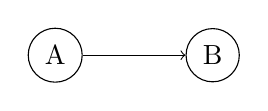
\begin{tikzpicture}
    \node (A) at (0,0) [circle, draw] {A};
    \node (B) at (2,0) [circle, draw] {B};
    \draw[->] (A) -- (B);
\end{tikzpicture}

In this graph:
- \(A\) and \(B\) are vertices (or nodes).
- The arrowed line between them represents an edge, indicating a directed relationship from \(A\) to \(B\).

\subsubsection{Degree of a Vertex}
Consider the following graph:

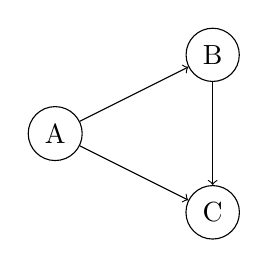
\begin{tikzpicture}
    \node (A) at (0,0) [circle, draw] {A};
    \node (B) at (2,1) [circle, draw] {B};
    \node (C) at (2,-1) [circle, draw] {C};
    \draw[->] (A) -- (B);
    \draw[->] (A) -- (C);
    \draw[->] (B) -- (C);
\end{tikzpicture}

In this graph:
- Vertex \(A\) has a degree of 2 because it has two edges connected to it (out-degree).
- Vertex \(B\) and vertex \(C\) each have a degree of 2, as each has two edges incident on them (one incoming and one outgoing edge).

\subsubsection{Path and Cycle}
Consider the following graph with a path and a cycle:

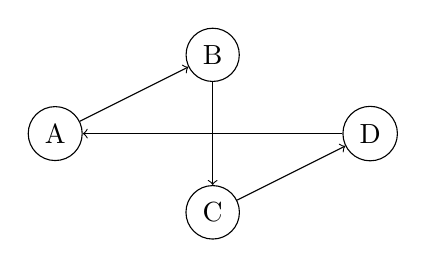
\begin{tikzpicture}
    \node (A) at (0,0) [circle, draw] {A};
    \node (B) at (2,1) [circle, draw] {B};
    \node (C) at (2,-1) [circle, draw] {C};
    \node (D) at (4,0) [circle, draw] {D};
    \draw[->] (A) -- (B);
    \draw[->] (B) -- (C);
    \draw[->] (C) -- (D);
    \draw[->] (D) -- (A); % cycle
\end{tikzpicture}

In this graph:
- The sequence \(A \rightarrow B \rightarrow C \rightarrow D\) represents a path.
- The edges \(A \rightarrow B \rightarrow C \rightarrow D \rightarrow A\) form a cycle because the path starts and ends at the same vertex, \(A\).

\subsubsection{Connected vs Disconnected Graph}
Here is an example of a connected graph:

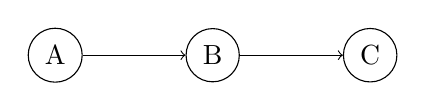
\begin{tikzpicture}
    \node (A) at (0,0) [circle, draw] {A};
    \node (B) at (2,0) [circle, draw] {B};
    \node (C) at (4,0) [circle, draw] {C};
    \draw[->] (A) -- (B);
    \draw[->] (B) -- (C);
\end{tikzpicture}

This graph is connected because there is a path between every pair of vertices.

Now, here is an example of a disconnected graph:

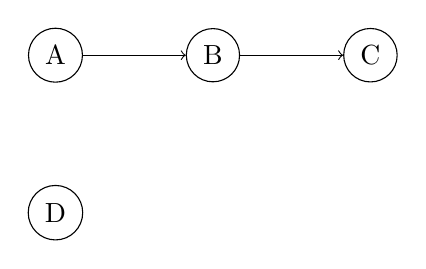
\begin{tikzpicture}
    \node (A) at (0,0) [circle, draw] {A};
    \node (B) at (2,0) [circle, draw] {B};
    \node (C) at (4,0) [circle, draw] {C};
    \node (D) at (0,-2) [circle, draw] {D};
    \draw[->] (A) -- (B);
    \draw[->] (B) -- (C);
\end{tikzpicture}

This graph is disconnected because there is no path between \(A, B, C\) and \(D\).


\subsection{Types of Graphs}

Graphs can be categorized in various ways, including:

\begin{itemize}
    \item \textbf{Directed Graph (Digraph)}: A \textbf{directed graph} (or \textbf{digraph}) is a graph where the edges have a direction. Each edge is an ordered pair of vertices, meaning that the edge from vertex \( u \) to vertex \( v \) is distinct from the edge from vertex \( v \) to vertex \( u \). This is useful when modeling situations where the relationship is asymmetric, such as in social media where one user follows another.
    
    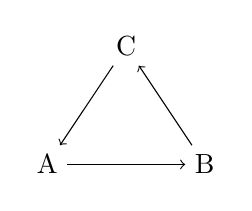
\begin{tikzpicture}
        \node (A) at (0,0) {A};
        \node (B) at (2,0) {B};
        \node (C) at (1,1.5) {C};
        
        \draw[->] (A) -- (B); % Directed edge A -> B
        \draw[->] (B) -- (C); % Directed edge B -> C
        \draw[->] (C) -- (A); % Directed edge C -> A
    \end{tikzpicture}

    \item \textbf{Undirected Graph}: An \textbf{undirected graph} is a graph where the edges do not have direction. An edge between vertices \( u \) and \( v \) is the same as an edge between \( v \) and \( u \). This type of graph is used when relationships between entities are bidirectional, such as friendships in social networks or two-way roads between cities.
    
    \begin{tikzpicture}
        \node (A) at (0,0) {A};
        \node (B) at (2,0) {B};
        \node (C) at (1,1.5) {C};
        
        \draw (A) -- (B); % Undirected edge A - B
        \draw (B) -- (C); % Undirected edge B - C
        \draw (C) -- (A); % Undirected edge C - A
    \end{tikzpicture}
    
    \item \textbf{Weighted Graph}: A \textbf{weighted graph} is a graph where each edge has a weight or cost associated with it. These weights often represent real-world quantities such as distance, time, or cost, and are useful in modeling situations like transport networks or logistical systems.
    
    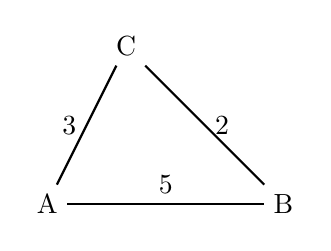
\begin{tikzpicture}
        \node (A) at (0,0) {A};
        \node (B) at (3,0) {B};
        \node (C) at (1,2) {C};
        
        \draw[thick] (A) -- (B) node[midway, above] {5}; % Weighted edge A - B with weight 5
        \draw[thick] (B) -- (C) node[midway, right] {2}; % Weighted edge B - C with weight 2
        \draw[thick] (C) -- (A) node[midway, left] {3}; % Weighted edge C - A with weight 3
    \end{tikzpicture}
    
    \item \textbf{Unweighted Graph}: An \textbf{unweighted graph} is a graph where edges do not have weights, representing simple connections without any associated cost or quantity. This type of graph is often used in theoretical studies or in simple problems where the connection itself is more important than the magnitude of the connection.
    
    \begin{tikzpicture}
        \node (A) at (0,0) {A};
        \node (B) at (2,0) {B};
        \node (C) at (1,1.5) {C};
        
        \draw (A) -- (B); % Unweighted edge A - B
        \draw (B) -- (C); % Unweighted edge B - C
        \draw (C) -- (A); % Unweighted edge C - A
    \end{tikzpicture}
    
    \item \textbf{Cyclic Graph}: A \textbf{cyclic graph} is a graph that contains at least one cycle. A cycle is a path that starts and ends at the same vertex, traversing through at least one other vertex. Cyclic graphs are often used to represent systems where elements have feedback loops, such as circuits or processes with recurring dependencies.
    
    \begin{tikzpicture}
        \node (A) at (0,0) {A};
        \node (B) at (2,0) {B};
        \node (C) at (1,1.5) {C};
        
        \draw (A) -- (B); % A - B
        \draw (B) -- (C); % B - C
        \draw (C) -- (A); % C - A (Cycle)
    \end{tikzpicture}
    
    \item \textbf{Acyclic Graph}: An \textbf{acyclic graph} is a graph that does not contain any cycles. If the graph is directed and acyclic, it is called a \textbf{Directed Acyclic Graph (DAG)}. Acyclic graphs are useful in modeling hierarchical structures or dependencies, such as task scheduling, version control systems, or data flow networks.
    
    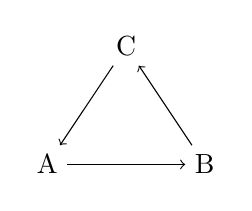
\begin{tikzpicture}
        \node (A) at (0,0) {A};
        \node (B) at (2,0) {B};
        \node (C) at (1,1.5) {C};
        
        \draw[->] (A) -- (B); % Directed edge A -> B
        \draw[->] (B) -- (C); % Directed edge B -> C
        \draw[->] (C) -- (A); % Directed edge C -> A (No cycle)
    \end{tikzpicture}
\end{itemize}

\subsection{Graph Traversal}

Graph traversal refers to the process of visiting all the vertices in a graph. The two primary methods for graph traversal are:

\begin{itemize}
    \item \textbf{Depth-First Search (DFS)}: DFS explores as far as possible along each branch before backtracking. It starts at a source vertex and recursively visits its neighbors. DFS can be implemented using recursion or a stack.
    \item \textbf{Breadth-First Search (BFS)}: BFS explores all neighbors of a vertex before moving on to the next level. It uses a queue to keep track of vertices to be explored. BFS is useful for finding the shortest path in an unweighted graph.
\end{itemize}

\twocolumn
\chapter{Graph Representations As Matrices}

\section{Matrices of Graphs}

In graph theory, matrices are often used to represent graphs, providing a compact and efficient way to store and manipulate graph data. The most common types of matrices used are the \textbf{adjacency matrix}, \textbf{incidence matrix}, and \textbf{degree matrix}. These matrices provide insight into the structure of the graph and allow us to perform operations such as traversal, finding paths, and determining connectivity.

\section{Adjacency Matrix}

The \textbf{adjacency matrix} is a square matrix used to represent a finite graph. The elements of the matrix indicate whether pairs of vertices are adjacent in the graph. 

- In an undirected graph, the adjacency matrix is symmetric, meaning that if there is an edge from vertex \(i\) to vertex \(j\), there is also an edge from vertex \(j\) to vertex \(i\).
- In a directed graph, the adjacency matrix is not necessarily symmetric, as edges have direction. An edge from vertex \(i\) to vertex \(j\) is represented by a non-zero entry in the matrix at position \((i, j)\).

\subsection{Formal Definition}

Let \( G = (V, E) \) be a graph with \(n\) vertices \(v_1, v_2, \dots, v_n\). The adjacency matrix \(A\) of the graph \(G\) is an \(n \times n\) matrix where the entry \(A_{ij}\) is:

\[
A_{ij} =
\begin{cases}
1 & \text{if there is an edge from vertex } v_i \text{ to vertex } v_j, \\
0 & \text{if there is no edge from vertex } v_i \text{ to vertex } v_j.
\end{cases}
\]

In the case of a directed graph, the adjacency matrix is defined as follows:

\[
A_{ij} = 
\begin{cases} 
1 & \text{if there is a directed edge from } v_i \text{ to } v_j, \\
0 & \text{if there is no directed edge from } v_i \text{ to } v_j.
\end{cases}
\]

\subsection{Example: Undirected Graph}

Consider a simple undirected graph with 3 vertices 

\(V = \{v_1, v_2, v_3\}\) and edges \(E = \{(v_1, v_2), (v_2, v_3)\}\). 

The adjacency matrix for this graph is:

\[
A = \begin{bmatrix}
0 & 1 & 0 \\
1 & 0 & 1 \\
0 & 1 & 0 \\
\end{bmatrix}
\]

This matrix shows that vertex \(v_1\) is connected to vertex \(v_2\) (hence \(A_{12} = 1\)) and vertex \(v_2\) is connected to vertex \(v_3\) (hence \(A_{23} = 1\)).

\subsection{Example: Directed Graph}

For a directed graph with 3 vertices \(V = \{v_1, v_2, v_3\}\) and edges \(E = \{(v_1, v_2), (v_2, v_3)\}\), the adjacency matrix would be:

\[
A = \begin{bmatrix}
0 & 1 & 0 \\
0 & 0 & 1 \\
0 & 0 & 0 \\
\end{bmatrix}
\]

Here, vertex \(v_1\) has a directed edge to vertex \(v_2\), and vertex \(v_2\) has a directed edge to vertex \(v_3\). The absence of edges from vertex \(v_3\) is reflected in the last row.

\section{Incidence Matrix}

The \textbf{incidence matrix} is another type of matrix used to represent a graph. It represents the relationship between vertices and edges. The rows of the matrix correspond to the vertices, while the columns correspond to the edges.

- In an undirected graph, an edge is incident to two vertices, and each edge is represented by two entries: \(+1\) and \(-1\) (or simply 1 if considering simple graphs).
- In a directed graph, the entries in the matrix are \(+1\) for the starting vertex (tail) of the edge, and \(-1\) for the ending vertex (head).

\subsection{Formal Definition}

Let \( G = (V, E) \) be a graph with \(n\) vertices and \(m\) edges. The incidence matrix \(B\) is an \(n \times m\) matrix where:

\[
B_{ij} =
\begin{cases}
1 & \text{if vertex } v_i \text{ is incident to edge } e_j, \\
-1 & \text{if vertex } v_i \text{ is the endpoint of directed edge } e_j, \\
0 & \text{if vertex } v_i \text{ is not incident to edge } e_j.
\end{cases}
\]

\subsection{Example: Directed Graph}

For a directed graph with 3 vertices and 2 edges \(V = \{v_1, v_2, v_3\}\) and \(E = \{e_1 = (v_1, v_2), e_2 = (v_2, v_3)\}\), the incidence matrix is:

\[
B = \begin{bmatrix}
1 & 0 \\
-1 & 1 \\
0 & -1 \\
\end{bmatrix}
\]

Here, the first column corresponds to edge \(e_1\) (from \(v_1\) to \(v_2\)), and the second column corresponds to edge \(e_2\) (from \(v_2\) to \(v_3\)).

\section{Degree Matrix}

The \textbf{degree matrix} is a diagonal matrix where each diagonal element represents the degree of the corresponding vertex in the graph.

- In an undirected graph, the degree of a vertex is simply the number of edges incident to it.
- In a directed graph, the degree can be split into in-degree (number of incoming edges) and out-degree (number of outgoing edges).

\subsection{Formal Definition}

For an undirected graph, the degree matrix \(D\) is a diagonal matrix where:

\[
D_{ii} = \text{degree of vertex } v_i
\]

For a directed graph, the degree matrix is typically split into two parts:

- \(D_{\text{in}}[ii] = \text{in-degree of vertex } v_i\)

- \(D_{\text{out}}[ii] = \text{out-degree of vertex } v_i\)

\subsection{Example: Degree Matrix for Undirected Graph}

Consider a graph with 3 vertices and edges

\(E = \{(v_1, v_2), (v_2, v_3), (v_1, v_3)\}\). The degree matrix for this graph is:

\[
D = \begin{bmatrix}
2 & 0 & 0 \\
0 & 2 & 0 \\
0 & 0 & 2 \\
\end{bmatrix}
\]

Each vertex has a degree of 2, as each is connected to two other vertices.

\section{Adjacency Matrix Representation For Undirected Graph}
This program demonstrates how an adjacency matrix is used to represent an undirected graph in C. An adjacency matrix is a square matrix used to represent a graph where the element at position \( M[i][j] \) is 1 if there is an edge between vertex \( i \) and vertex \( j \), and 0 if there is no edge. 

In this program, a graph with 5 vertices and 3 edges is used, and the adjacency matrix is updated based on the edges defined in the input.

The code performs the following key tasks:
\begin{itemize}
    \item Initializes the adjacency matrix with zeros.
    \item Inserts edges into the matrix, making the corresponding entries 1.
    \item Displays the adjacency matrix.
    \item Lists the edges of the graph in terms of vertex pairs.
\end{itemize}

\subsection{Code}

\begin{verbatim}
#define MAX 5
typedef int AdjMatrix[MAX][MAX];

void initMatrix(AdjMatrix M);
void insertEdge(AdjMatrix M, int edge[2]);
void displayMatrix(AdjMatrix M);
void displayEdges(AdjMatrix M);

int main() {
    int edges[][2] = {{1, 2}, {2, 3}, {3, 0}};
    int numOfEdges = sizeof(edges) / sizeof(edges[0]);
    
    AdjMatrix M;
    initMatrix(M);

    for(int i = 0; i < numOfEdges; i++) {
        insertEdge(M, edges[i]);
    }

    displayMatrix(M);
    displayEdges(M);
}

void initMatrix(AdjMatrix M) {
    for(int i = 0; i < MAX; i++) {
        for(int j = 0; j < MAX; j++) {
            M[i][j] = 0;
        }
    }
}

void insertEdge(AdjMatrix M, int edge[2]) {
    M[edge[0]][edge[1]] = 1;
    M[edge[1]][edge[0]] = 1;
}

void displayMatrix(AdjMatrix M) {
    for(int i = 0; i < MAX; i++) {
        for(int j = 0; j < MAX; j++) {
            printf("%d ", M[i][j]);
        }
        printf("\n");
    }
}

void displayEdges(AdjMatrix M) {
    printf("Edges: ");
    for(int i = 0; i < MAX; i++) {
        for(int j = i + 1; j < MAX; j++) {
            if(M[i][j] == 1) {
                printf("(%d, %d) ", i, j);
            }
        }
    }
}
\end{verbatim}

\subsection{Graph Representation Example}
Given the edges \((1, 2)\), \((2, 3)\), and \((3, 0)\), the adjacency matrix would look like the following:

\begin{figure}[h!]
    \centering
    \begin{tabular}{|c|c|c|c|c|}
    \hline
    0 & 1 & 0 & 0 & 0 \\
    \hline
    1 & 0 & 1 & 0 & 0 \\
    \hline
    0 & 1 & 0 & 1 & 0 \\
    \hline
    0 & 0 & 1 & 0 & 0 \\
    \hline
    0 & 0 & 0 & 0 & 0 \\
    \hline
    \end{tabular}
    \caption{Adjacency Matrix for the Graph with Vertices 0, 1, 2, 3, 4 and Edges (1, 2), (2, 3), (3, 0)}
\end{figure}

In this matrix:
\begin{itemize}
    \item The entry \texttt{M[0][1] = 1} and \texttt{M[1][0] = 1} represents an edge between vertex 0 and vertex 1.
    \item The entry \texttt{M[1][2] = 1} and \texttt{M[2][1] = 1} represents an edge between vertex 1 and vertex 2.
    \item The entry \texttt{M[2][3] = 1} and \texttt{M[3][2] = 1} represents an edge between vertex 2 and vertex 3.
    \item The remaining entries are 0, indicating no edge between the corresponding vertices.
\end{itemize}

The edges of the graph are:
\[
(0, 1), (1, 2), (2, 3)
\]

\subsection{Execution Flow}
1. The program initializes a 5x5 adjacency matrix with all zero values.
2. It then inserts three edges: (0, 1), (1, 2), and (2, 3), marking the respective matrix entries with 1.
3. The adjacency matrix is displayed, showing the connections between vertices.
4. The edges are then displayed in the form of vertex pairs.

\twocolumn

\section{Adjacency Matrix for Directed Graph in C}
This program demonstrates the representation of a directed graph using an adjacency matrix in C. An adjacency matrix is used to represent the relationships (edges) between vertices (nodes) in a graph. In a directed graph, an edge from vertex \( i \) to vertex \( j \) is represented by setting the matrix entry \( M[i][j] \) to 1. The matrix entry \( M[j][i] \) is not affected unless there is a reverse edge from \( j \) to \( i \).

In this specific example, we have a directed graph with 5 vertices and 3 edges, and we use an adjacency matrix to represent the graph's connections. The program performs the following tasks:
\begin{itemize}
    \item Initializes an adjacency matrix with zeros.
    \item Inserts directed edges into the matrix.
    \item Displays the adjacency matrix.
    \item Lists the directed edges of the graph.
\end{itemize}

The key parts of the code are explained below:

\begin{verbatim}
#define MAX 5
typedef int AdjMatrix[MAX][MAX];

void initMatrix(AdjMatrix M);
void insertEdge(AdjMatrix M, int edge[2]);
void displayMatrix(AdjMatrix M);
void displayEdges(AdjMatrix M);

int main() {
    int edges[][2] = {{1, 2}, {2, 3}, {3, 0}};
    int numOfEdges = sizeof(edges) / sizeof(edges[0]);
    
    AdjMatrix M;
    initMatrix(M);

    for(int i = 0; i < numOfEdges; i++) {
        insertEdge(M, edges[i]);
    }

    displayMatrix(M);
    displayEdges(M);
}

void initMatrix(AdjMatrix M) {
    for(int i = 0; i < MAX; i++) {
        for(int j = 0; j < MAX; j++) {
            M[i][j] = 0;
        }
    }
}

void insertEdge(AdjMatrix M, int edge[2]) {
    M[edge[0]][edge[1]] = 1;
}

void displayMatrix(AdjMatrix M) {
    for(int i = 0; i < MAX; i++) {
        for(int j = 0; j < MAX; j++) {
            printf("%d ", M[i][j]);
        }
        printf("\n");
    }
}

void displayEdges(AdjMatrix M) {
    printf("Edges: ");
    for(int i = 0; i < MAX; i++) {
        for(int j = 0; j < MAX; j++) {
            if(M[i][j] == 1) {
                printf("(%d, %d) ", i, j);
            }
        }
    }
}
\end{verbatim}

\subsection{Graph Representation Example}
Given the directed edges \((1, 2)\), \((2, 3)\), and \((3, 0)\), the adjacency matrix would be as follows:

\begin{figure}[h!]
    \centering
    \begin{tabular}{|c|c|c|c|c|}
    \hline
    0 & 1 & 0 & 0 & 0 \\
    \hline
    0 & 0 & 1 & 0 & 0 \\
    \hline
    0 & 0 & 0 & 1 & 0 \\
    \hline
    1 & 0 & 0 & 0 & 0 \\
    \hline
    0 & 0 & 0 & 0 & 0 \\
    \hline
    \end{tabular}
    \caption{Adjacency Matrix for Directed Graph with Vertices 0, 1, 2, 3, 4 and Edges (1, 2), (2, 3), (3, 0)}
\end{figure}

In this matrix:
\begin{itemize}
    \item The entry \texttt{M[1][2] = 1} represents a directed edge from vertex 1 to vertex 2.
    \item The entry \texttt{M[2][3] = 1} represents a directed edge from vertex 2 to vertex 3.
    \item The entry \texttt{M[3][0] = 1} represents a directed edge from vertex 3 to vertex 0.
    \item All other entries remain 0, indicating no directed edge exists between those vertices.
\end{itemize}

\subsection{Execution Flow}
1. The program initializes a 5x5 adjacency matrix with zeros.
2. It inserts three directed edges: (1, 2), (2, 3), and (3, 0), setting the respective matrix entries to 1.
3. The adjacency matrix is displayed, showing the directed connections between vertices.
4. The directed edges are then displayed as pairs of vertices.


\chapter{Graph Algorithms: Searching}

\section{Breadth-First Search (BFS) with Queue Implementation}

The provided code implements the **Breadth-First Search (BFS)** algorithm on a graph, represented by an adjacency matrix. Additionally, a **queue** is used to handle the nodes being processed during BFS. In this program, the graph is limited to 5 nodes, denoted by the constant \texttt{MAX}. The BFS algorithm traverses the graph level by level, visiting all the neighbors of a node before moving on to the next level.

\subsection{Key Concepts}

\begin{itemize}
    \item \textbf{Adjacency Matrix:} An adjacency matrix is a 2D array used to represent a graph. Each cell \texttt{M[i][j]} is \texttt{1} if there is an edge between nodes \texttt{i} and \texttt{j}, and \texttt{0} otherwise. This matrix allows efficient checking for the presence of edges.
    \item \textbf{Queue for BFS:} The BFS algorithm uses a queue to ensure nodes are processed in the correct order. The queue guarantees that nodes are visited level by level.
    \item \textbf{Bit-Vector for Visited Nodes:} A bit-vector (implemented as an integer array) is used to keep track of which nodes have been visited during the BFS traversal. This prevents revisiting nodes.
\end{itemize}

\subsection{Code Walkthrough}

The following sections break down the major components and functions in the code:

\subsubsection{Adjacency Matrix Initialization}

The adjacency matrix \texttt{M} is initialized to zero, meaning there are initially no edges between nodes. The function \texttt{initMatrix} sets all the matrix elements to \texttt{0}.

\begin{verbatim}
void initMatrix(AdjMatrix M) {
    for (int i = 0; i < MAX; i++) {
        for (int j = 0; j < MAX; j++) {
            M[i][j] = 0;
        }
    }
}
\end{verbatim}

\subsubsection{Inserting Edges}

The function \texttt{insertEdge} modifies the adjacency matrix to reflect an edge between two nodes. For an undirected graph, both \texttt{M[edge[0]][edge[1]]} and \texttt{M[edge[1]][edge[0]]} are set to \texttt{1}, indicating the presence of an edge.

\begin{verbatim}
void insertEdge(AdjMatrix M, int edge[2]) {
    M[edge[0]][edge[1]] = 1;
    M[edge[1]][edge[0]] = 1;
}
\end{verbatim}

\subsubsection{BFS Traversal}

BFS begins by marking the root node as visited. The algorithm then processes nodes level by level, starting with the root node. The \texttt{visited} bit-vector ensures that each node is only visited once. Nodes are enqueued for processing, and their neighbors are added to the queue if they haven't been visited already.

\begin{verbatim}
void bfs(AdjMatrix M, int root) {
    Set visited = {};
    visited[root] = 1;
    
    Queue Q;
    initQueue(&Q);
    
    enqueue(&Q, root);
    
    printf("BFS: ");
    
    while (!isEmpty(Q)) {
        int node = dequeue(&Q);
        printf("%d ", node);
        
        for (int i = 0; i < MAX; i++) {
            if (visited[i] == 0 && M[node][i] != 0) {
                visited[i] = 1;
                enqueue(&Q, i);
            }
        }
    }
}
\end{verbatim}

\subsubsection{Queue Implementation}

A queue is used in BFS to manage nodes that need to be processed. The queue is implemented as a circular queue with two pointers, \texttt{front} and \texttt{rear}.

\begin{verbatim}
typedef struct {
    int nodes[MAX];
    int front;
    int rear;
} Queue; // Array-based queue implementation
\end{verbatim}

The following functions handle the queue operations:
- \texttt{initQueue}: Initializes the queue.
- \texttt{isEmpty}: Checks if the queue is empty.
- \texttt{enqueue}: Adds a node to the queue.
- \texttt{dequeue}: Removes a node from the front of the queue.

\begin{verbatim}
void initQueue(Queue *Q) {
    Q->front = 1;
    Q->rear = 0;
}

bool isEmpty(Queue Q) {
    return (Q.rear + 1) % MAX == Q.front ? true : false;
}

void enqueue(Queue *Q, int data) {
    if ((Q->rear + 2) % MAX != Q->front) {
        Q->rear = (Q->rear + 1) % MAX;
        Q->nodes[Q->rear] = data;
    }
}

int dequeue(Queue *Q) {
    int ret = -1;
    if (!isEmpty(*Q)) {
        ret = Q->nodes[Q->front];
        Q->front = (Q->front + 1) % MAX;
    }
    return ret;
}
\end{verbatim}

\subsubsection{Matrix and Edge Display}

The function \texttt{displayMatrix} prints the adjacency matrix, allowing the user to visualize the graph's structure. The function \texttt{displayEdges} iterates through the matrix to print all edges present in the graph.

\begin{verbatim}
void displayMatrix(AdjMatrix M) {
    for (int i = 0; i < MAX; i++) {
        for (int j = 0; j < MAX; j++) {
            printf("%d ", M[i][j]);
        }
        printf("\n");
    }
}

void displayEdges(AdjMatrix M) {
    printf("Edges: ");
    for (int i = 0; i < MAX; i++) {
        for (int j = i + 1; j < MAX; j++) {
            if (M[i][j] == 1) {
                printf("(%d, %d) ", i, j);
            }
        }
    }
    printf("\n");
}
\end{verbatim}

\subsection{Example Output}

For the given graph with edges \{(0, 1), (1, 4), (1, 2), (2, 3), (3, 4)\}, the adjacency matrix might look like this:

\[
\begin{bmatrix}
0 & 1 & 0 & 0 & 0 \\
1 & 0 & 1 & 0 & 1 \\
0 & 1 & 0 & 1 & 0 \\
0 & 0 & 1 & 0 & 1 \\
0 & 1 & 0 & 1 & 0 \\
\end{bmatrix}
\]

The BFS traversal starting from node \texttt{0} would output:

\[
\text{BFS: } 0, 1, 4, 2, 3
\]

\section{Depth-First Search (DFS) on a Graph Using an Adjacency Matrix}

This program demonstrates the application of Depth-First Search (DFS) on a graph represented using an adjacency matrix. DFS is an algorithm for traversing or searching tree or graph data structures. It starts at a root node and explores as far as possible along each branch before backtracking.

In this specific program:
\begin{itemize}
    \item The graph is represented using an adjacency matrix.
    \item The DFS algorithm is implemented using a recursive approach.
    \item The program uses a set (bit-vector) to keep track of visited nodes during the traversal.
    \item The program initializes the matrix, inserts edges, displays the adjacency matrix, and performs DFS starting from a given root node.
\end{itemize}

The key parts of the code are explained below:

\begin{verbatim}
#define MAX 5
typedef int Set[MAX]; // bit-vector
typedef int AdjMatrix[MAX][MAX];

void dfs(AdjMatrix M, Set visited, int root);
void initMatrix(AdjMatrix M);
void insertEdge(AdjMatrix M, int edge[2]);
void displayMatrix(AdjMatrix M);
void displayEdges(AdjMatrix M);

int main() {
    int edges[][2] = {{0, 1}, {1, 4}, {1, 2}, {2, 3}, {3, 4}};
    int numOfEdges = sizeof(edges) / sizeof(edges[0]);
    
    AdjMatrix M;
    initMatrix(M);

    for(int i = 0; i < numOfEdges; i++) {
        insertEdge(M, edges[i]);
    }

    displayMatrix(M);
    displayEdges(M);

    int root = 0;
    Set visited = {};

    printf("DFS: ");
    dfs(M, visited, root);

    return 0;
}

void dfs(AdjMatrix M, Set visited, int root) {
    printf("%d ", root);
    visited[root] = 1;

    for(int i = 0; i < MAX; i++) {
        if(visited[i] == 0 && M[root][i] != 0) {
            dfs(M, visited, i);
        }
    }
}

void initMatrix(AdjMatrix M) {
    for(int i = 0; i < MAX; i++) {
        for(int j = 0; j < MAX; j++) {
            M[i][j] = 0;
        }
    }
}

void insertEdge(AdjMatrix M, int edge[2]) {
    M[edge[0]][edge[1]] = 1;
    M[edge[1]][edge[0]] = 1; // For an undirected graph
}

void displayMatrix(AdjMatrix M) {
    for(int i = 0; i < MAX; i++) {
        for(int j = 0; j < MAX; j++) {
            printf("%d ", M[i][j]);
        }
        printf("\n");
    }
}

void displayEdges(AdjMatrix M) {
    printf("Edges: ");
    for(int i = 0; i < MAX; i++) {
        for(int j = i + 1; j < MAX; j++) {
            if(M[i][j] == 1) {
                printf("(%d, %d) ", i, j);
            }
        }
    }
    printf("\n");
}
\end{verbatim}

\subsection{Graph Representation and DFS Algorithm}

The graph in this program consists of 5 vertices labeled 0 through 4, and 5 edges:
\[
(0, 1), (1, 4), (1, 2), (2, 3), (3, 4)
\]
The adjacency matrix representation of the graph is as follows:

\begin{figure}[h!]
    \centering
    \begin{tabular}{|c|c|c|c|c|}
    \hline
    0 & 1 & 0 & 0 & 0 \\
    \hline
    1 & 0 & 1 & 0 & 1 \\
    \hline
    0 & 1 & 0 & 1 & 0 \\
    \hline
    0 & 0 & 1 & 0 & 1 \\
    \hline
    0 & 1 & 0 & 1 & 0 \\
    \hline
    \end{tabular}
    \caption{Adjacency Matrix for the Graph with Vertices 0, 1, 2, 3, 4 and Edges (0, 1), (1, 4), (1, 2), (2, 3), (3, 4)}
\end{figure}

In the adjacency matrix:
\begin{itemize}
    \item The entry \texttt{M[0][1] = 1} indicates an edge from vertex 0 to vertex 1.
    \item The entry \texttt{M[1][4] = 1} indicates an edge from vertex 1 to vertex 4.
    \item The entry \texttt{M[1][2] = 1} indicates an edge from vertex 1 to vertex 2.
    \item The entry \texttt{M[2][3] = 1} indicates an edge from vertex 2 to vertex 3.
    \item The entry \texttt{M[3][4] = 1} indicates an edge from vertex 3 to vertex 4.
    \item The matrix is symmetric because the graph is undirected; each edge is represented in both directions (i.e., \texttt{M[i][j]} and \texttt{M[j][i]}).
\end{itemize}

\subsection{DFS Traversal}

The DFS traversal algorithm works by starting at a given root node and exploring as deeply as possible along each branch before backtracking. The visited nodes are tracked using a set (bit-vector). The traversal follows these steps:
\begin{itemize}
    \item Start from the root node (in this case, node 0).
    \item Visit the node and mark it as visited.
    \item Move to an adjacent node (if unvisited) and continue the process recursively.
    \item Backtrack when no unvisited adjacent nodes are left.
\end{itemize}

For the graph represented above, the DFS starting from node 0 would visit the nodes in the following order: \texttt{0, 1, 2, 3, 4}.

\subsection{Visualization of DFS Traversal}

In this example, starting from node 0:
\begin{itemize}
    \item Node 0 is visited first, then the algorithm moves to node 1.
    \item From node 1, the algorithm moves to node 2.
    \item From node 2, the algorithm moves to node 3.
    \item From node 3, the algorithm moves to node 4, which has no unvisited neighbors.
    \item All nodes have been visited, so the traversal ends.
\end{itemize}

The output would look like this:
\[
\text{DFS: } 0 \ 1 \ 2 \ 3 \ 4
\]
\thispagestyle{empty}
\chapter{Graph Algorithms: Finding The Shortest Paths}

\section{Dijkstra's Algorithm: Deep Dive}

Dijkstra's algorithm is a classic algorithm used for finding the shortest paths from a source node to all other nodes in a graph, assuming all edge weights are non-negative. In this section, we explore the implementation of Dijkstra's algorithm in C, detailing each key component and providing a thorough explanation of the underlying concepts.

\subsection{Graph Representation: Adjacency Matrix}

In the provided C code, the graph is represented using an \textbf{Adjacency Matrix} (denoted as \( M \)). The adjacency matrix is a two-dimensional array where each entry \( M[i][j] \) contains the weight of the edge connecting node \( i \) and node \( j \). If there is no edge between two nodes, the matrix entry holds a special value, in this case, \(\infty\) (represented as \texttt{INF}), indicating the absence of a direct connection. 

This is particularly useful in a graph where all nodes are expected to be directly connected to each other, as it allows efficient retrieval of the weight of any edge in constant time. The matrix is initialized with \(\infty\) for non-existent edges, and the actual edge weights are inserted via the \texttt{insertEdge} function.

The adjacency matrix representation of the graph will look like this:

\[
\begin{bmatrix}
\infty & 2 & 4 & \infty & \infty \\
2 & \infty & 1 & 7 & \infty \\
4 & 1 & \infty & \infty & 3 \\
\infty & 7 & \infty & \infty & 2 \\
\infty & \infty & 3 & 2 & \infty
\end{bmatrix}
\]

In the matrix above, each row and column corresponds to a node in the graph. For example, the weight of the edge from node 0 to node 1 is 2, as seen in \( M[0][1] = 2 \).

\subsection{Key Variables and Data Structures}

The key variables and data structures used in the algorithm include:

\begin{itemize}
    \item \textbf{Set visited}: A bit vector used to track whether a node has been visited or not during the execution of the algorithm. It is initialized such that only the root node is marked as visited at the beginning.
    \item \textbf{weightFromRoot[]}: An array storing the current shortest distance from the root node to every other node. This array is updated during the algorithm as shorter paths are discovered.
    \item \textbf{Set}: A typedef for the bit vector implementation, which has a size of \texttt{MAX} (5 in this case), representing the maximum number of nodes in the graph.
\end{itemize}

\subsection{Initialization: Setting Up the Graph}

The function \texttt{initMatrix(AdjMatrix M)} initializes the adjacency matrix by setting all values to \texttt{INF}, indicating that no edges exist initially between any pairs of nodes. This matrix will later be populated with actual edge weights using the \texttt{insertEdge} function. 

Each edge is represented as an array \texttt{edge[3]}, where the first two elements are the nodes connected by the edge and the third element is the weight of the edge. For example, \texttt{edge[0] = 0}, \texttt{edge[1] = 1}, and \texttt{edge[2] = 2} represent an edge between node 0 and node 1 with a weight of 2.

\subsection{Dijkstra’s Algorithm Execution}

The function \texttt{dijkstras(AdjMatrix M, int root)} implements the core of Dijkstra’s algorithm. The algorithm works by iteratively visiting the nearest unvisited node and updating the shortest path to its neighbors.

The steps are as follows:
\begin{enumerate}
    \item Initialize the \texttt{visited} set to mark the root node as visited.
    \item Set the initial distances from the root to all other nodes. These distances are taken directly from the adjacency matrix, representing the direct edges from the root node.
    \item In each iteration, find the unvisited node with the smallest distance (using the \texttt{smallestIndex} variable). Mark this node as visited.
    \item Update the distances of the neighbors of the newly visited node by checking if a shorter path exists through the current node.
    \item Repeat the process until all nodes have been visited.
\end{enumerate}

The array \texttt{weightFromRoot[]} is updated during each iteration to reflect the shortest path found from the root node to each of the other nodes.

\subsection{Displaying the Results}

The function \texttt{displayDjk(int arr[], int root)} displays the results of Dijkstra’s algorithm. It prints the shortest distance from the root node to each of the other nodes. If no path exists to a particular node (i.e., the value is still \(\infty\)), it prints \texttt{NONE}.

The output shows the shortest paths from the root node to each node, allowing you to easily verify the correctness of the algorithm.

\subsection{Example Execution}

Given the graph with the following edges:
\begin{itemize}
    \item \( (0, 1, 2) \)
    \item \( (0, 2, 4) \)
    \item \( (1, 2, 1) \)
    \item \( (1, 3, 7) \)
    \item \( (2, 4, 3) \)
    \item \( (4, 3, 2) \)
\end{itemize}

The adjacency matrix representation of the graph will be:

\[
\begin{bmatrix}
\infty & 2 & 4 & \infty & \infty \\
2 & \infty & 1 & 7 & \infty \\
4 & 1 & \infty & \infty & 3 \\
\infty & 7 & \infty & \infty & 2 \\
\infty & \infty & 3 & 2 & \infty
\end{bmatrix}
\]

After running Dijkstra’s algorithm with node 0 as the root, the shortest paths to all other nodes are as follows:

\begin{itemize}
    \item From node 0 to node 1: 2
    \item From node 0 to node 2: 3
    \item From node 0 to node 3: 7
    \item From node 0 to node 4: 6
\end{itemize}

\onecolumn
\subsection{Code}
\begin{verbatim}
    #include <stdio.h>
#include <stdlib.h>
#define MAX 5
#define INF 9999

typedef int Set[MAX]; // bit-vector implementation
typedef int AdjMatrix[MAX][MAX];

int* dijkstras(AdjMatrix M, int root);
void displayDjk(int arr[], int root);
void initMatrix(AdjMatrix M);
void insertEdge(AdjMatrix M, int edge[3]);
void displayMatrix(AdjMatrix M);

int main() {
    int edges[][3] = {
        {0, 1, 2},  // Edge from 0 to 1 with weight 2
        {0, 2, 4},  // Edge from 0 to 2 with weight 4
        {1, 2, 1},  // Edge from 1 to 2 with weight 1
        {1, 3, 7},  // Edge from 1 to 3 with weight 7
        {2, 4, 3},  // Edge from 2 to 4 with weight 3
        {4, 3, 2}   // Edge from 4 to 3 with weight 2
    };

    int numOfEdges = sizeof(edges) / sizeof(edges[0]);
    
    AdjMatrix M;
    initMatrix(M);

    for(int i = 0; i < numOfEdges; i++) {
        insertEdge(M, edges[i]);
    }

    displayMatrix(M);

    int root = 0;
    int *djk = dijkstras(M, root);
    displayDjk(djk, root);

    return 0;
}

int* dijkstras(AdjMatrix M, int root) {
    int *weightFromRoot = (int*) malloc(sizeof(int) * MAX);
    
    if(weightFromRoot != NULL) {
        Set visited = {};
        visited[root] = 1; 

        // initialize weight from root
        for(int i = 0; i < MAX; i++) {
            weightFromRoot[i] = M[root][i];
        }

        weightFromRoot[root] = 0;

        // algorithm
        for(int i = 1; i < MAX; i++) {
            int smallestIndex = 0;

            // find smallest
            for(int j = 0; j < MAX; j++) {
                if(visited[smallestIndex] == 1
                || (weightFromRoot[j] < weightFromRoot[smallestIndex] && visited[j] == 0)) {
                    smallestIndex = j;
                }
            }

            // add smallestIndex to visited
            visited[smallestIndex] = 1;

            for(int k = 0; k < MAX; k++) {
                if(visited[k] == 0) {
                    int nextWeight = weightFromRoot[smallestIndex] + M[smallestIndex][k]; 
                    // adds the new path from smallestIndex to next index
                    weightFromRoot[k] = (weightFromRoot[k] < nextWeight) ? weightFromRoot[k] : nextWeight;
                    // new weight gets the lesser of the two
                }
            }
        }
    }

    return weightFromRoot;
}

void displayDjk(int arr[], int root) {
    printf("\nDijkstra's Paths from %d:\n", root);
    for(int i = 0; i < MAX; i++) {
        
        printf("Path from %d to %d: ", root, i);
        (arr[i] == INF) ? printf("NONE\n") : printf("%d\n", arr[i]);
    }
}

void initMatrix(AdjMatrix M) {
    for(int i = 0; i < MAX; i++) {
        for(int j = 0; j < MAX; j++) {
            M[i][j] = INF; // initialized to INF if not adjacent
        }
    }
}

void insertEdge(AdjMatrix M, int edge[3]) {
    M[edge[0]][edge[1]] = edge[2];
    M[edge[1]][edge[0]] = edge[2];
}

void displayMatrix(AdjMatrix M) {
    for(int i = 0; i < MAX; i++) {
        for(int j = 0; j < MAX; j++) {
            (M[i][j] == INF) ? printf("INF ") : printf("%3d ", M[i][j]);
        }
        printf("\n");
    }
}
\end{verbatim}
\twocolumn
\section{Floyd-Warshall Algorithm: Deep Dive}

The Floyd-Warshall algorithm is a classic dynamic programming approach used to find the shortest paths between all pairs of nodes in a weighted graph. In this section, we explore the implementation of the Floyd-Warshall algorithm in C, breaking down the key components and the underlying logic.

\subsection{Graph Representation: Adjacency Matrix}

Similar to Dijkstra’s algorithm, the graph in this implementation is represented using an \textbf{Adjacency Matrix}, where each element \( M[i][j] \) contains the weight of the edge between node \( i \) and node \( j \). If no edge exists between two nodes, the value is set to a special constant \(\infty\) (represented as \texttt{INF} in the code), which indicates no direct path between those nodes. 

The adjacency matrix is initialized with all values set to \(\infty\), except for the diagonal elements (representing the self-loops), which are set to 0.

The adjacency matrix for the graph with the following edges:

\begin{itemize}
    \item \( (0, 1, 2) \)
    \item \( (0, 2, 4) \)
    \item \( (1, 2, 1) \)
    \item \( (1, 3, 7) \)
    \item \( (2, 4, 3) \)
    \item \( (4, 3, 2) \)
\end{itemize}

is represented as:

\[
\begin{bmatrix}
\infty & 2 & 4 & \infty & \infty \\
2 & \infty & 1 & 7 & \infty \\
4 & 1 & \infty & \infty & 3 \\
\infty & 7 & \infty & \infty & 2 \\
\infty & \infty & 3 & 2 & \infty
\end{bmatrix}
\]

Here, each cell \( M[i][j] \) represents the weight of the edge from node \( i \) to node \( j \). If no edge exists between \( i \) and \( j \), the value is set to \(\infty\).

\subsection{Key Variables and Data Structures}

The algorithm makes use of the following variables and data structures:

\begin{itemize}
    \item \textbf{AdjMatrix M}: A 2D array representing the graph, initialized with \(\infty\) for non-adjacent nodes.
    \item \textbf{weights[][]}: A dynamically allocated 2D array used to store the shortest path distances between all pairs of nodes during the execution of the algorithm.
    \item \textbf{INF}: A constant representing infinity, used to indicate no direct connection between nodes.
\end{itemize}

\subsection{Floyd-Warshall Algorithm Implementation}

The function \texttt{floyds(AdjMatrix M)} implements the core logic of the Floyd-Warshall algorithm. It initializes the distance matrix by copying the initial adjacency matrix \( M \), setting the diagonal elements to 0 (distance to itself). The algorithm then proceeds by updating the matrix in three nested loops to compute the shortest paths between all pairs of nodes.

The key idea behind Floyd-Warshall is that for each pair of nodes \( i \) and \( j \), the algorithm checks if the path from \( i \) to \( j \) through an intermediate node \( k \) is shorter than the direct path. If so, the matrix is updated with the shorter distance.

\begin{enumerate}
    \item For each pair of nodes \( i \) and \( j \), check if a shorter path exists through an intermediate node \( k \).
    \item Update the distance matrix with the shortest path between any two nodes.
    \item Repeat until the shortest paths are found for all pairs of nodes.
\end{enumerate}

The function \texttt{floyds()} operates in \( O(n^3) \) time, where \( n \) is the number of nodes in the graph, due to the three nested loops.

\subsection{Displaying the Results}

The function \texttt{displayFloyds(int **flyd)} prints the resulting shortest path matrix after running the Floyd-Warshall algorithm. If a distance is still set to \(\infty\), it prints \texttt{INF} to indicate no path exists between the nodes.

\subsection{Initialization and Insertion of Edges}

The functions \texttt{initMatrix(AdjMatrix M)} and \texttt{insertEdge(AdjMatrix M, int edge[3])} are used to initialize the graph matrix and insert edges, respectively. 

\texttt{initMatrix(AdjMatrix M)} initializes all elements of the adjacency matrix to \(\infty\) (indicating no edges), except for the diagonal elements which are set to 0. 

\texttt{insertEdge(AdjMatrix M, int edge[3])} takes an array representing an edge between two nodes and updates the adjacency matrix to reflect the edge’s weight. The graph is assumed to be undirected, so the matrix is updated symmetrically.

\subsection{Example Execution}

Given the graph with the edges defined earlier, the initial adjacency matrix is:

\[
\begin{bmatrix}
\infty & 2 & 4 & \infty & \infty \\
2 & \infty & 1 & 7 & \infty \\
4 & 1 & \infty & \infty & 3 \\
\infty & 7 & \infty & \infty & 2 \\
\infty & \infty & 3 & 2 & \infty
\end{bmatrix}
\]

After running the Floyd-Warshall algorithm, the shortest paths between all pairs of nodes are computed, resulting in the following matrix:

\[
\begin{bmatrix}
0 & 2 & 3 & 6 & 6 \\
2 & 0 & 1 & 4 & 4 \\
3 & 1 & 0 & 5 & 3 \\
6 & 4 & 5 & 0 & 2 \\
6 & 4 & 3 & 2 & 0
\end{bmatrix}
\]

\onecolumn
\begin{verbatim}
    #include <stdio.h>
#include <stdlib.h>
#define MAX 5
#define INF 9999

typedef int AdjMatrix[MAX][MAX];

int **floyds(AdjMatrix M);
void displayFloyds(int **flyd);
void initMatrix(AdjMatrix M);
void insertEdge(AdjMatrix M, int edge[3]);
void displayMatrix(AdjMatrix M);

int main() {
    int edges[][3] = {
        {0, 1, 2},  // Edge from 0 to 1 with weight 2
        {0, 2, 4},  // Edge from 0 to 2 with weight 4
        {1, 2, 1},  // Edge from 1 to 2 with weight 1
        {1, 3, 7},  // Edge from 1 to 3 with weight 7
        {2, 4, 3},  // Edge from 2 to 4 with weight 3
        {4, 3, 2}   // Edge from 4 to 3 with weight 2
    };

    int numOfEdges = sizeof(edges) / sizeof(edges[0]);
    
    AdjMatrix M;
    initMatrix(M);

    for(int i = 0; i < numOfEdges; i++) {
        insertEdge(M, edges[i]);
    }

    displayMatrix(M);

    int root = 0;
    int **flyd= floyds(M);
    displayFloyds(flyd);

    return 0;
}

int **floyds(AdjMatrix M) {
    int **weights = (int**) malloc(sizeof(int*) * MAX);

    // initialize weights
    for(int i = 0; i < MAX; i++){
        weights[i] = (int*) malloc(sizeof(int) * MAX);

        // copy to M
        for(int j = 0; j < MAX; j++) {
            if(i == j) {
                weights[i][j] = 0;
            }
            else {
                weights[i][j] = M[i][j];
            }
        }
    }


    // algorithm O(n^3)
    for(int k = 0; k < MAX; k++) { // connecting vertex
        for(int i = 0; i < MAX; i++) { // source vertex
            for(int j = 0; j < MAX; j++) { // destination vertex
                int newWeight = weights[i][k] + weights[k][j];

                if(newWeight < weights[i][j]) {
                    weights[i][j] = newWeight;
                } 
            }
        }
    }

    return weights;
}

void displayFloyds(int **flyd) {
    for(int i = 0; i < MAX; i++) {
        for(int j = 0; j < MAX; j++) {
            (flyd[i][j] == INF) ? printf("INF ") : printf("%3d ", flyd[i][j]);
        }
        printf("\n");
    }
    printf("\n");
} 

void initMatrix(AdjMatrix M) {
    for(int i = 0; i < MAX; i++) {
        for(int j = 0; j < MAX; j++) {
            M[i][j] = INF; // initialized to INF if not adjacent
        }
    }
}

void insertEdge(AdjMatrix M, int edge[3]) {
    M[edge[0]][edge[1]] = edge[2];
    M[edge[1]][edge[0]] = edge[2];
}

void displayMatrix(AdjMatrix M) {
    for(int i = 0; i < MAX; i++) {
        for(int j = 0; j < MAX; j++) {
            (M[i][j] == INF) ? printf("INF ") : printf("%3d ", M[i][j]);
        }
        printf("\n");
    }
    printf("\n");
}
\end{verbatim}

\twocolumn
\section{Warshall's Algorithm: Deep Dive}

Warshall's algorithm computes the transitive closure of a graph, which identifies whether there exists a path between two nodes. This is typically used in graph theory to determine reachability within a graph. In this section, we break down the implementation of Warshall's algorithm in C, focusing on the key components and their functionality.

\subsection{Graph Representation: Adjacency Matrix}

Similar to other graph algorithms, Warshall’s algorithm represents the graph using an \textbf{Adjacency Matrix}. Each element \( M[i][j] \) in this matrix contains a value indicating whether there is a direct edge from node \( i \) to node \( j \). If no edge exists, the value is set to a special constant \(\infty\) (represented as \texttt{INF} in the code). If there is an edge between the nodes, the value is set to 1.

The adjacency matrix is initialized such that all non-diagonal values are set to \(\infty\), representing no direct paths, while the diagonal elements (representing self-loops) are set to 0, indicating that the distance to a node itself is zero.

\subsection{Key Variables and Data Structures}

The algorithm utilizes the following data structures:

\begin{itemize}
    \item \textbf{AdjMatrix M}: A 2D array representing the graph, initialized with \(\infty\) for non-adjacent nodes.
    \item \textbf{weights[][]}: A dynamically allocated 2D array used to store the reachability information between all pairs of nodes.
    \item \textbf{INF}: A constant used to represent infinity, which indicates no direct connection between nodes.
\end{itemize}

\subsection{Warshall's Algorithm Implementation}

The function \texttt{warshalls(AdjMatrix M)} implements the core logic of Warshall's algorithm. It first initializes the weights matrix by copying the original adjacency matrix \( M \), and then iteratively updates the matrix to reflect the transitive closure.

The key idea behind Warshall's algorithm is that for each pair of nodes \( i \) and \( j \), the algorithm checks if there is an indirect path between them through an intermediate node \( k \). If such a path exists, the matrix is updated to reflect that a path from \( i \) to \( j \) is now reachable.

\begin{enumerate}
    \item For each pair of nodes \( i \) and \( j \), check if a path exists through an intermediate node \( k \).
    \item Update the matrix to indicate whether there is a path between nodes \( i \) and \( j \).
    \item Repeat the process until the transitive closure is complete for all pairs of nodes.
\end{enumerate}

The function \texttt{warshalls()} operates in \( O(n^3) \) time complexity, where \( n \) is the number of nodes, due to the three nested loops.

\subsection{Displaying the Results}

The function \texttt{displayWarshalls(int **warsh)} prints the resulting reachability matrix after executing Warshall's algorithm. If a value is still set to \(\infty\), it prints \texttt{INF} to indicate that no path exists between the nodes.

\subsection{Initialization and Insertion of Edges}

The functions \texttt{initMatrix(AdjMatrix M)} and \texttt{insertEdge(AdjMatrix M, int edge[2])} are used to initialize the graph matrix and insert edges, respectively.

\texttt{initMatrix(AdjMatrix M)} initializes all elements of the adjacency matrix to \(\infty\) (indicating no edges), except for the diagonal elements, which are set to 0.

\texttt{insertEdge(AdjMatrix M, int edge[2])} takes an array representing an edge between two nodes and updates the adjacency matrix to reflect the presence of an edge. The graph is assumed to be undirected, so the matrix is updated symmetrically.

\subsection{Example Execution}

Given the graph with the following edges:

\begin{itemize}
    \item \( (0, 1) \)
    \item \( (0, 2) \)
    \item \( (1, 2) \)
    \item \( (1, 3) \)
    \item \( (2, 4) \)
    \item \( (4, 3) \)
\end{itemize}

The initial adjacency matrix is:

\[
\begin{bmatrix}
\infty & 1 & 1 & \infty & \infty \\
1 & \infty & 1 & 1 & \infty \\
1 & 1 & \infty & \infty & 1 \\
\infty & 1 & \infty & \infty & 1 \\
\infty & \infty & 1 & 1 & \infty
\end{bmatrix}
\]

After running Warshall's algorithm, the reachability matrix (transitive closure) is computed, resulting in:

\[
\begin{bmatrix}
0 & 1 & 1 & 1 & 1 \\
1 & 0 & 1 & 1 & 1 \\
1 & 1 & 0 & 1 & 1 \\
1 & 1 & 1 & 0 & 1 \\
1 & 1 & 1 & 1 & 0
\end{bmatrix}
\]

This matrix shows that all nodes are reachable from any other node, indicating full connectivity within the graph.

\onecolumn
\begin{verbatim}
    #include <stdio.h>
#include <stdlib.h>
#define MAX 5
#define INF 9999

typedef int AdjMatrix[MAX][MAX];

int **warshalls(AdjMatrix M);
void displayWarshalls(int **warsh);
void initMatrix(AdjMatrix M);
void insertEdge(AdjMatrix M, int edge[2]);
void displayMatrix(AdjMatrix M);

int main() {
    int edges[][2] = {
        {0, 1},  // Edge from 0 to 1 
        {0, 2},  // Edge from 0 to 2 
        {1, 2},  // Edge from 1 to 2 
        {1, 3},  // Edge from 1 to 3
        {2, 4},  // Edge from 2 to 4
        {4, 3}   // Edge from 4 to 3
    };

    int numOfEdges = sizeof(edges) / sizeof(edges[0]);
    
    AdjMatrix M;
    initMatrix(M);

    for(int i = 0; i < numOfEdges; i++) {
        insertEdge(M, edges[i]);
    }

    displayMatrix(M);

    int **warsh = warshalls(M);
    displayWarshalls(warsh);

    return 0;
}

int **warshalls(AdjMatrix M) {
    int **weights = (int**) malloc(sizeof(int*) * MAX);

    // initialize weights
    for(int i = 0; i < MAX; i++){
        weights[i] = (int*) malloc(sizeof(int) * MAX);

        // copy to M
        for(int j = 0; j < MAX; j++) {
            if(i == j) {
                weights[i][j] = 0;
            }
            else {
                weights[i][j] = M[i][j];
            }
        }
    }


    // algorithm O(n^3)
    for(int k = 0; k < MAX; k++) { // connecting vertex
        for(int i = 0; i < MAX; i++) { // source vertex
            for(int j = 0; j < MAX; j++) { // destination vertex
                if(weights[i][k] == 1 && weights[k][j] == 1) { 
                    // if there is a path from i to k, 
                    and a path from k to j, then there is a path from i to j
                    weights[i][j] = 1;
                } 
            }
        }
    }

    return weights;
}

void displayWarshalls(int **warsh) {
    for(int i = 0; i < MAX; i++) {
        for(int j = 0; j < MAX; j++) {
            (warsh[i][j] == INF) ? printf("INF ") : printf("%3d ", warsh[i][j]);
        }
        printf("\n");
    }
    printf("\n");
} 

void initMatrix(AdjMatrix M) {
    for(int i = 0; i < MAX; i++) {
        for(int j = 0; j < MAX; j++) {
            M[i][j] = INF; // initialized to INF if not adjacent
        }
    }
}

void insertEdge(AdjMatrix M, int edge[2]) {
    M[edge[0]][edge[1]] = 1;
    M[edge[1]][edge[0]] = 1;
}

void displayMatrix(AdjMatrix M) {
    for(int i = 0; i < MAX; i++) {
        for(int j = 0; j < MAX; j++) {
            (M[i][j] == INF) ? printf("INF ") : printf("%3d ", M[i][j]);
        }
        printf("\n");
    }
    printf("\n");
}
\end{verbatim}

\twocolumn
\chapter{Graph Algorithms: Minimum Cost Spanning Trees}
\section{Kruskal's Algorithm for Minimum Spanning Tree (MST)}

The function \texttt{kruskAlgo} implements Kruskal's Algorithm to find the Minimum Spanning Tree (MST) of a graph. It uses a Min-Heap to store edges sorted by weight, and progressively selects edges to form the MST while ensuring no cycles are created. Below is a detailed explanation of the function:

\subsection{Data Structure Definitions}
\begin{verbatim}
typedef int graphType[MAX][MAX];
typedef int set[MAX]; 

typedef struct {
	int u, v; 
	int weight; 
}edgetype;

typedef struct {
	edgetype heap[HEAPMAX];
	int count;
} minHeap;

typedef struct {
    edgetype edges[MAX];
	int minCost;
	int count;
}kruskMST;

\end{verbatim}

\newpage
\subsection{Code}

\begin{verbatim}
kruskMST kruskAlgo(minHeap* heap)
{
    kruskMST k = {.minCost = 0, .count = 0};

    int comp[6];
    
    int i;
    for(i = 0; i < MAX; i++){
        comp[i] = i;
    }

    while(heap->count > 0){
        edgetype min = deleteMin(heap);
        
        if(comp[min.u] != comp[min.v]){
            int change = comp[min.u];

            for(i = 0; i < MAX; i++){
                if(comp[i] == change){
                    comp[i] = comp[min.v];
                }
            }
            
            k.edges[k.count++] = min;
            k.minCost += min.weight;
        }
    }
    
    return k;
}
\end{verbatim}

\twocolumn



\newpage
\onecolumn
\subsection{Step 1: Initialize the Kruskal's MST Structure}

We begin by initializing a structure to store the MST and its associated cost:

\begin{verbatim}
kruskMST k = {.minCost = 0, .count = 0};
\end{verbatim}

Here:
- \texttt{k.minCost} is set to 0, and it will hold the total cost of the MST once it is calculated.
- \texttt{k.count} starts at 0 and will keep track of the number of edges added to the MST.

\subsection{Step 2: Initialize the Components Array}

Next, we initialize an array \texttt{comp} where each vertex is initially its own parent:

\begin{verbatim}
int comp[6];
for(i = 0; i < MAX; i++) {
    comp[i] = i;
}
\end{verbatim}

The array \texttt{comp[i]} represents the parent of vertex \(i\). Initially, each vertex is its own parent, indicating that all vertices are in separate connected components.

\subsection{Step 3: Process Edges from the Min-Heap}

We then enter a loop where we process edges from the Min-Heap. As long as there are edges left in the heap, we select the edge with the smallest weight:

\begin{verbatim}
while(heap->count > 0) {
    edgetype min = deleteMin(heap);
\end{verbatim}

Here, the \texttt{deleteMin(heap)} function removes and returns the edge with the smallest weight from the heap.

\subsection{Step 4: Check for Cycles (Disjoint Set Union)}

Before adding the selected edge to the MST, we check if it would form a cycle. This is done by comparing the connected components (parents) of the two vertices of the edge:

\begin{verbatim}
if(comp[min.u] != comp[min.v]) {
    int change = comp[min.u];
\end{verbatim}

If the two vertices \(u\) and \(v\) are in different components (i.e., \texttt{comp[min.u] != comp[min.v]}), then adding the edge does not form a cycle, and we can safely add it to the MST.

\subsection{Step 5: Merge the Components}

Once we confirm that the edge does not form a cycle, we merge the two components by updating the parent of all vertices in the same component as \texttt{min.u}:

\begin{verbatim}
for(int i = 0; i < MAX; i++) {
    if(comp[i] == change) {
        comp[i] = comp[min.v];
    }
}
\end{verbatim}

This loop ensures that all vertices in the same connected component as \(u\) now belong to the component of \(v\), effectively merging the two components.

\subsection{Step 6: Add the Edge to the MST}

Now that the edge is safe to add to the MST, we do so by updating the MST structure:

\begin{verbatim}
k.edges[k.count++] = min;
k.minCost += min.weight;
\end{verbatim}

Here:
- \texttt{k.edges[k.count++]} adds the edge \texttt{min} to the MST.
- \texttt{k.minCost} is updated by adding the weight of the edge \texttt{min.weight}.

\subsection*{Step 7: Return the Minimum Spanning Tree}

Finally, the function returns the MST stored in the \texttt{k} structure:

\begin{verbatim}
return k;
\end{verbatim}

\section{Kruskal's Algorithm: Before and After}

\subsection{Before Kruskal's Algorithm}

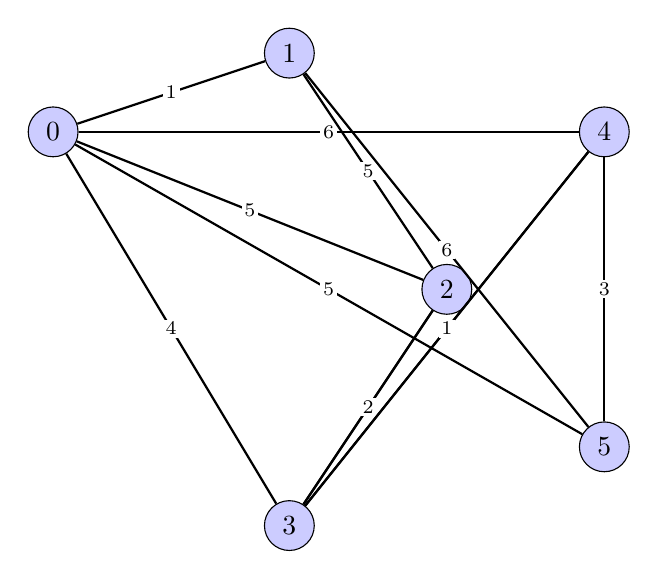
\begin{tikzpicture}[
    vertex/.style={circle, draw, fill=blue!20, inner sep=2pt, minimum size=18pt},
    edge/.style={draw, thick},
    weight/.style={font=\scriptsize, midway, fill=white, inner sep=1pt}
]

% Define vertices in a different layout
\node[vertex] (0) at (0, 2) {0};
\node[vertex] (1) at (3, 3) {1};
\node[vertex] (2) at (5, 0) {2};
\node[vertex] (3) at (3, -3) {3};
\node[vertex] (4) at (7, 2) {4};
\node[vertex] (5) at (7, -2) {5};

% Define edges with weights
\path[edge] (0) -- node[weight] {1} (1);
\path[edge] (0) -- node[weight] {5} (2);
\path[edge] (0) -- node[weight] {4} (3);
\path[edge] (0) -- node[weight] {6} (4);
\path[edge] (0) -- node[weight] {5} (5);
\path[edge] (1) -- node[weight] {5} (2);
\path[edge] (1) -- node[weight] {6} (5);
\path[edge] (2) -- node[weight] {2} (3);
\path[edge] (3) -- node[weight] {2} (2); % Redundant edge in undirected graph
\path[edge] (3) -- node[weight] {1} (4);
\path[edge] (4) -- node[weight] {1} (3); % Redundant edge in undirected graph
\path[edge] (4) -- node[weight] {3} (5);

\end{tikzpicture}

\subsection{After Kruskal's Algorithm}

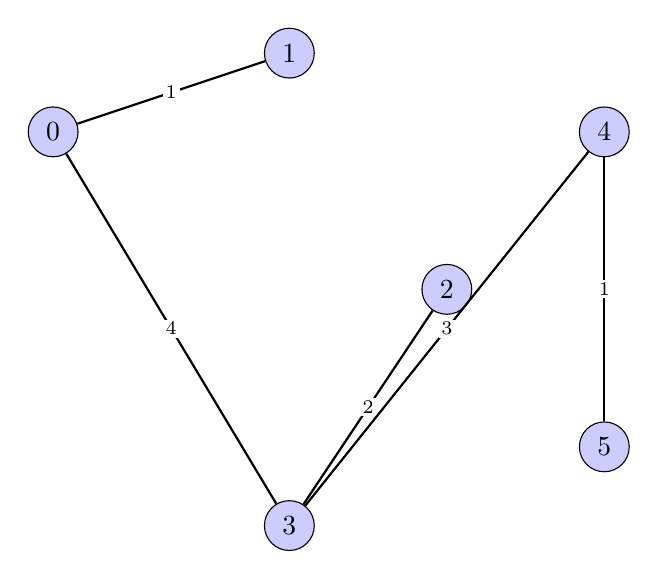
\begin{tikzpicture}[
    vertex/.style={circle, draw, fill=blue!20, inner sep=2pt, minimum size=18pt},
    edge/.style={draw, thick},
    weight/.style={font=\scriptsize, midway, fill=white, inner sep=1pt}
]

% Define vertices in the same layout
\node[vertex] (0) at (0, 2) {0};
\node[vertex] (1) at (3, 3) {1};
\node[vertex] (2) at (5, 0) {2};
\node[vertex] (3) at (3, -3) {3};
\node[vertex] (4) at (7, 2) {4};
\node[vertex] (5) at (7, -2) {5};

% Define edges for MST
\path[edge] (0) -- node[weight] {1} (1);
\path[edge] (2) -- node[weight] {2} (3);
\path[edge] (3) -- node[weight] {3} (4);
\path[edge] (0) -- node[weight] {4} (3);
\path[edge] (4) -- node[weight] {1} (5);

\end{tikzpicture}

\subsection{Summary}

In summary, Kruskal's algorithm processes edges in increasing order of weight, checking whether each edge connects two different components. If it does, the edge is added to the MST, and the two components are merged. This process continues until the MST contains \( |V| - 1 \) edges, where \( |V| \) is the number of vertices.

The time complexity of this implementation is \(O(E \log E)\), where \(E\) is the number of edges, because of the heap operations and sorting of the edges

\newpage
\twocolumn
\section{Flight Network Optimization}

This C program implements Kruskal's algorithm to find the Minimum Spanning Tree (MST) of a graph, where cities are represented as vertices and flights between cities are represented as edges. The goal of Kruskal’s algorithm is to connect all the cities with the minimum total flight cost, while avoiding any cycles in the graph. 

The program starts by taking input from the user, which includes the number of cities, the number of flights, and the details of each flight (source city, destination city, and cost). Once the input is gathered, Kruskal’s algorithm is applied to compute the MST.

The sections below explain the key components and the step-by-step execution of the program.

\subsection{Data Structures Used}

The program uses two main data structures to represent the problem:

\begin{itemize}
    \item \textbf{Flight Structure:} The \texttt{Flight} structure is used to represent a flight between two cities. It contains the following fields:
    \begin{itemize}
        \item \texttt{source}: The source city of the flight.
        \item \texttt{destination}: The destination city of the flight.
        \item \texttt{cost}: The cost of the flight.
    \end{itemize}

    \item \textbf{Subset Structure:} The \texttt{Subset} structure is used to keep track of the connected components (or sets of cities) during the algorithm. It contains:
    \begin{itemize}
        \item \texttt{parent}: The parent city of the subset, which is used to track the representative of the set.
        \item \texttt{rank}: The rank (or depth) of the subset. It is used to help optimize the union operation by always attaching the smaller tree to the root of the larger tree, reducing the overall height of the tree.
    \end{itemize}
\end{itemize}

\subsection{Function Descriptions}

The program consists of several functions, each with a specific purpose. Here is an overview:

\begin{itemize}
    \item \textbf{compareFlights:} This function compares two flights based on their costs. It is used for sorting the flights in increasing order of cost. Sorting the flights is important because Kruskal's algorithm processes the edges in ascending order of their weights (costs).
    
    \item \textbf{find:} This function is used to find the root of a set (city) in the union-find structure. It uses path compression to optimize future queries by directly linking elements to the root of the set, speeding up the algorithm.
    
    \item \textbf{unionSets:} This function merges two subsets into one. It uses the union by rank technique, where the smaller set (determined by rank) is attached to the larger set to keep the tree flat and efficient.
    
    \item \textbf{kruskalMST:} This is the main function that implements Kruskal's algorithm. It sorts the flights by cost, then iterates over the sorted flights to add edges to the MST, ensuring that no cycles are formed using the union-find operations. It outputs the final MST and the total cost.
\end{itemize}

\subsection{Step-by-Step Breakdown of Kruskal's Algorithm}

Let’s walk through how Kruskal's algorithm works in this program:

\begin{enumerate}
    \item \textbf{Input:} 
    The user is prompted to input the number of cities and flights, followed by the details of each flight (source, destination, and cost). This data is stored in an array of \texttt{Flight} structures.
    
    \item \textbf{Sorting the Flights:}
    Once the flight data is collected, the program sorts the flights by cost in ascending order. This is done using the \texttt{compareFlights} function, which compares the cost of two flights and ensures that the cheapest flights are processed first. Sorting the edges is a crucial step in Kruskal’s algorithm because it ensures we always add the least expensive edge first.
    
    \item \textbf{Initialize Union-Find:}
    The next step is to initialize the union-find data structure. Each city starts as its own subset (set), and the rank is set to 0 for all cities. The \texttt{parent} of each subset is initially the city itself.
    
    \item \textbf{Processing Flights:}
    Now, the algorithm starts processing the sorted flights. For each flight:
    \begin{itemize}
        \item The \texttt{find} function is used to check if the source and destination cities of the flight are in the same subset. If they are in the same subset, adding the flight would create a cycle, so we skip this flight.
        \item If the source and destination cities are not in the same subset (i.e., they are not connected yet), the flight is added to the MST, and the \texttt{unionSets} function is used to combine the subsets of the source and destination cities.
    \end{itemize}

    \item \textbf{Stopping Condition:}
    The algorithm stops once we have added \texttt{numCities - 1} edges to the MST. This is the minimum number of edges required to connect all cities in the graph. If we finish processing all the flights and the MST does not contain \texttt{numCities - 1} edges, it indicates that the graph is disconnected, and an MST cannot be formed.
    
    \item \textbf{Output:}
    After constructing the MST, the program outputs the edges in the MST along with their costs, followed by the total cost of the MST. If the graph is disconnected, a message is displayed indicating that no MST can be formed.
\end{enumerate}

\subsection{Example Run}

Let’s walk through a brief example to understand how this works.

\begin{enumerate}
    \item The user enters 4 cities and 5 flights.
    \item The flight data is entered as follows:
    \begin{itemize}
        \item Flight 1: Source = 0, Destination = 1, Cost = 10
        \item Flight 2: Source = 1, Destination = 2, Cost = 20
        \item Flight 3: Source = 0, Destination = 2, Cost = 15
        \item Flight 4: Source = 2, Destination = 3, Cost = 5
        \item Flight 5: Source = 1, Destination = 3, Cost = 25
    \end{itemize}
    \item The flights are sorted by cost: (5, 10, 15, 20, 25).
    \item The union-find structure starts with each city as its own subset.
    \item Kruskal’s algorithm proceeds by adding the edges with the lowest costs, ensuring no cycles form, until the MST contains 3 edges (since 4 cities require 3 edges to be connected).
    \item The program prints the MST:
    \begin{itemize}
        \item Edge 2-3 with cost 5
        \item Edge 0-1 with cost 10
        \item Edge 0-2 with cost 15
    \end{itemize}
    \item The total cost of the MST is 30.
\end{enumerate}

\subsection{Edge Case: Disconnected Graph}

In some cases, the graph may not be fully connected, meaning it is impossible to form a spanning tree. For example, if there are fewer than \texttt{numCities - 1} edges after processing all flights, the program will detect that the graph is disconnected and print a message saying, "The graph is not fully connected; MST cannot be formed."


\newpage


\twocolumn
\section{Prim's Algorithm\\(non-POT implementation)}

Prim's Algorithm is a greedy algorithm that finds the minimum spanning tree (MST) for a weighted, connected, and undirected graph. The algorithm starts from an arbitrary vertex and iteratively adds the smallest edge connecting a visited vertex to an unvisited vertex, ensuring that the resulting tree has the minimum possible weight.
\subsection{Data Structure Definitions}

\begin{verbatim}
typedef int graphType[MAX][MAX];
typedef int set[MAX]; 

typedef struct {
	int u, v; 
	int weight;
}edgetype;

typedef struct {
    edgetype edges[MAX];
    int edgeCount;
	int minCost;
}primMST;
\end{verbatim}

\newpage

\subsection{Code}
\begin{verbatim}
primMST primAlgo(graphType graph, int startVertex)
{
	primMST p = {.edgeCount = 0, .minCost = 0};
	set visited = {};
	visited[startVertex] = 1;

	int i, j;

	while(p.edgeCount < MAX - 1){
		
		edgetype minEdge = {.weight = INFINITY};

		for(i = 0; i < MAX; i++){
			if(visited[i] == 1){
			
				for(j = 0; j < MAX; j++){
					if(visited[j] == 0 && graph[i][j] < minEdge.weight){
						edgetype temp = {i, j, graph[i][j]};
						minEdge = temp;
					}
				}
			}
		}

		p.minCost += minEdge.weight;
		
		if(minEdge.weight != INFINITY){
			p.edges[p.edgeCount++] = minEdge;
			visited[minEdge.v] = 1;
		} else {
			printf("Graph is not connected");
		}
	}
	return p;
}
\end{verbatim}



\onecolumn
\subsection{Step 1: Initialize the Prim's MST Structure}

We begin by initializing a structure to store the MST and its associated cost:

\begin{verbatim}
primMST p = {.edgeCount = 0, .minCost = 0};
\end{verbatim}

Here:
- \texttt{p.edgeCount} is set to 0 and will keep track of the number of edges added to the MST.
- \texttt{p.minCost} is also initialized to 0, and it will store the total weight of the MST once it is computed.

\subsection{Step 2: Initialize the Visited Set}

Next, we initialize a set \texttt{visited} to track which vertices have been added to the MST:

\begin{verbatim}
set visited = {};
visited[startVertex] = 1;
\end{verbatim}

Here:
- \texttt{visited[startVertex] = 1;} marks the starting vertex as visited, indicating the starting point for the MST.
- The set \texttt{visited} will be used to check which vertices have already been added to the MST.

\subsection{Step 3: Process Edges to Find the Minimum Edge}

We then enter a loop that continues until the MST contains \(V - 1\) edges (where \(V\) is the number of vertices in the graph). In each iteration, we find the smallest edge that connects a visited vertex to an unvisited vertex:

\begin{verbatim}
while(p.edgeCount < MAX - 1) {
    edgetype minEdge = {.weight = INFINITY};
\end{verbatim}

Here:
- We initialize \texttt{minEdge} with an infinite weight to ensure that any valid edge found will be smaller.
- The loop continues until we have added \(V - 1\) edges to the MST.

\subsection{Step 4: Check Each Edge for Minimum Weight}

Inside the loop, we iterate through all vertices to find the smallest edge connecting a visited vertex to an unvisited one:

\begin{verbatim}
for(i = 0; i < MAX; i++) {
    if(visited[i] == 1) {
        for(j = 0; j < MAX; j++) {
            if(visited[j] == 0 && graph[i][j] < minEdge.weight) {
                edgetype temp = {i, j, graph[i][j]};
                minEdge = temp;
            }
        }
    }
}
\end{verbatim}

Here:
- For each visited vertex \(i\), we check all unvisited vertices \(j\).
- If the weight of the edge between \(i\) and \(j\) is smaller than the current \texttt{minEdge}, we update \texttt{minEdge} to store this new minimum edge.

\subsection{Step 5: Add the Minimum Edge to the MST}

Once the minimum edge is found, we update the MST structure and the total cost:

\begin{verbatim}
p.minCost += minEdge.weight;
\end{verbatim}

Here:
- We add the weight of the selected \texttt{minEdge} to \texttt{p.minCost}, which tracks the total cost of the MST.

\subsection{Step 6: Mark the Vertex as Visited and Add Edge to MST}

Now that we have selected the minimum edge, we mark the destination vertex of the edge as visited and add the edge to the MST:

\begin{verbatim}
if(minEdge.weight != INFINITY) {
    p.edges[p.edgeCount++] = minEdge;
    visited[minEdge.v] = 1;
} else {
    printf("Graph is not connected");
}
\end{verbatim}

Here:
- The edge \texttt{minEdge} is added to the MST in \texttt{p.edges[p.edgeCount++]}.
- The destination vertex \texttt{minEdge.v} is marked as visited.
- If no valid edge is found, it indicates that the graph is disconnected, and we print an error message.

\subsection{Step 7: Return the Minimum Spanning Tree}

Finally, the function returns the MST stored in the structure \texttt{p}:

\begin{verbatim}
return p;
\end{verbatim}

\section{Graph and MST}

\subsection{Original Graph Matrix}

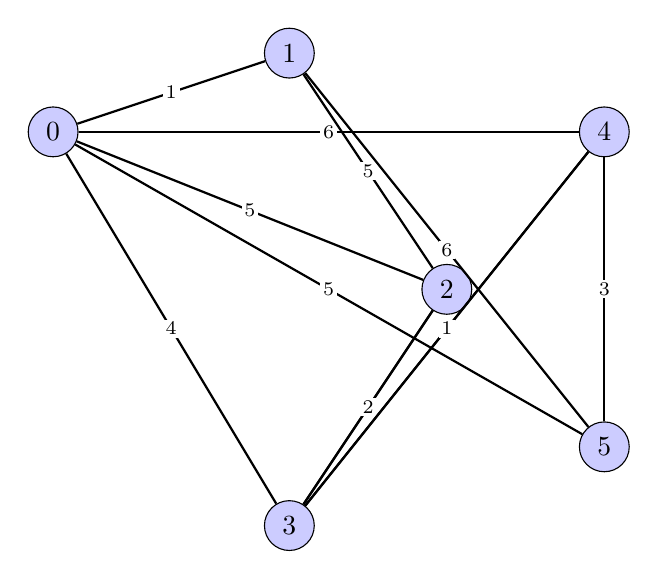
\begin{tikzpicture}[
    vertex/.style={circle, draw, fill=blue!20, inner sep=2pt, minimum size=18pt},
    edge/.style={draw, thick},
    weight/.style={font=\scriptsize, midway, fill=white, inner sep=1pt}
]

% Define vertices
\node[vertex] (0) at (0, 2) {0};
\node[vertex] (1) at (3, 3) {1};
\node[vertex] (2) at (5, 0) {2};
\node[vertex] (3) at (3, -3) {3};
\node[vertex] (4) at (7, 2) {4};
\node[vertex] (5) at (7, -2) {5};

% Define edges with weights
\path[edge] (0) -- node[weight] {1} (1);
\path[edge] (0) -- node[weight] {5} (2);
\path[edge] (0) -- node[weight] {4} (3);
\path[edge] (0) -- node[weight] {6} (4);
\path[edge] (0) -- node[weight] {5} (5);
\path[edge] (1) -- node[weight] {5} (2);
\path[edge] (1) -- node[weight] {6} (5);
\path[edge] (2) -- node[weight] {2} (3);
\path[edge] (3) -- node[weight] {2} (2); % Redundant edge in undirected graph
\path[edge] (3) -- node[weight] {1} (4);
\path[edge] (4) -- node[weight] {1} (3); % Redundant edge in undirected graph
\path[edge] (4) -- node[weight] {3} (5);

\end{tikzpicture}

\subsection{Minimum Spanning Tree (MST)}

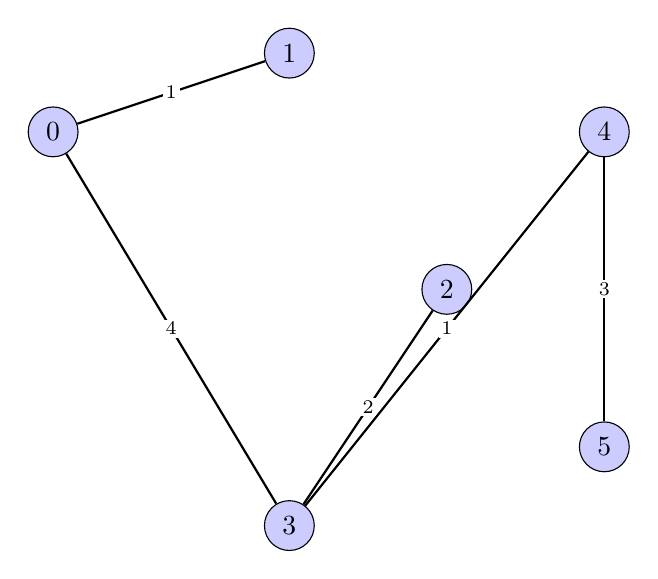
\begin{tikzpicture}[
    vertex/.style={circle, draw, fill=blue!20, inner sep=2pt, minimum size=18pt},
    edge/.style={draw, thick},
    weight/.style={font=\scriptsize, midway, fill=white, inner sep=1pt}
]

% Define vertices
\node[vertex] (0) at (0, 2) {0};
\node[vertex] (1) at (3, 3) {1};
\node[vertex] (2) at (5, 0) {2};
\node[vertex] (3) at (3, -3) {3};
\node[vertex] (4) at (7, 2) {4};
\node[vertex] (5) at (7, -2) {5};

% Define edges for MST
\path[edge] (1) -- node[weight] {1} (0); % (1, 0) = 1
\path[edge] (0) -- node[weight] {4} (3); % (0, 3) = 4
\path[edge] (3) -- node[weight] {1} (4); % (3, 4) = 1
\path[edge] (3) -- node[weight] {2} (2); % (3, 2) = 2
\path[edge] (4) -- node[weight] {3} (5); % (4, 5) = 3

\end{tikzpicture}

\subsection{Summary}

In summary, Prim's Algorithm finds the minimum spanning tree (MST) by iteratively selecting the smallest edge that connects a visited vertex to an unvisited vertex. The process continues until all vertices are included in the MST. The total cost of the MST is tracked as the sum of the weights of the selected edges.

The time complexity of this implementation is \(O(V^2)\), where \(V\) is the number of vertices, due to the nested loops. This can be improved to \(O(E \log V)\) by using a priority queue to select the minimum edge more efficiently.


\end{document}
